\documentclass[tikz,border=8pt]{standalone}
% Shared look for every TikZ diagram. Load with % Shared look for every TikZ diagram. Load with % Shared look for every TikZ diagram. Load with \input{../../tools/tikz-style.tex}
\usepackage[T1]{fontenc}
\usepackage{lmodern}
\renewcommand{\sfdefault}{lmr}  % diagrams use the same serif as the text
\usetikzlibrary{arrows.meta, positioning, shapes.geometric, calc, fit, backgrounds}
\definecolor{cblue}{HTML}{4C78A8}
\definecolor{corange}{HTML}{F58518}
\definecolor{cgreen}{HTML}{54A24B}
\definecolor{cred}{HTML}{E45756}
\definecolor{cpurple}{HTML}{B279A2}
\definecolor{cgrey}{HTML}{6B6B6B}
\tikzset{
  every picture/.style={font=\sffamily, line width=1.2pt},
  box/.style={draw=#1, fill=#1!12, rounded corners=4pt, align=center, inner sep=7pt, minimum height=1.1cm},
  box/.default=cgrey,
  arrow/.style={-{Stealth[length=3mm]}, draw=cgrey, line width=1.4pt},
  title/.style={font=\sffamily\bfseries\Large},
  note/.style={font=\sffamily\small, text=cgrey, align=center},
}
\AtBeginDocument{\hyphenpenalty=10000 \exhyphenpenalty=10000}

\usepackage[T1]{fontenc}
\usepackage{lmodern}
\renewcommand{\sfdefault}{lmr}  % diagrams use the same serif as the text
\usetikzlibrary{arrows.meta, positioning, shapes.geometric, calc, fit, backgrounds}
\definecolor{cblue}{HTML}{4C78A8}
\definecolor{corange}{HTML}{F58518}
\definecolor{cgreen}{HTML}{54A24B}
\definecolor{cred}{HTML}{E45756}
\definecolor{cpurple}{HTML}{B279A2}
\definecolor{cgrey}{HTML}{6B6B6B}
\tikzset{
  every picture/.style={font=\sffamily, line width=1.2pt},
  box/.style={draw=#1, fill=#1!12, rounded corners=4pt, align=center, inner sep=7pt, minimum height=1.1cm},
  box/.default=cgrey,
  arrow/.style={-{Stealth[length=3mm]}, draw=cgrey, line width=1.4pt},
  title/.style={font=\sffamily\bfseries\Large},
  note/.style={font=\sffamily\small, text=cgrey, align=center},
}
\AtBeginDocument{\hyphenpenalty=10000 \exhyphenpenalty=10000}

\usepackage[T1]{fontenc}
\usepackage{lmodern}
\renewcommand{\sfdefault}{lmr}  % diagrams use the same serif as the text
\usetikzlibrary{arrows.meta, positioning, shapes.geometric, calc, fit, backgrounds}
\definecolor{cblue}{HTML}{4C78A8}
\definecolor{corange}{HTML}{F58518}
\definecolor{cgreen}{HTML}{54A24B}
\definecolor{cred}{HTML}{E45756}
\definecolor{cpurple}{HTML}{B279A2}
\definecolor{cgrey}{HTML}{6B6B6B}
\tikzset{
  every picture/.style={font=\sffamily, line width=1.2pt},
  box/.style={draw=#1, fill=#1!12, rounded corners=4pt, align=center, inner sep=7pt, minimum height=1.1cm},
  box/.default=cgrey,
  arrow/.style={-{Stealth[length=3mm]}, draw=cgrey, line width=1.4pt},
  title/.style={font=\sffamily\bfseries\Large},
  note/.style={font=\sffamily\small, text=cgrey, align=center},
}
\AtBeginDocument{\hyphenpenalty=10000 \exhyphenpenalty=10000}

\begin{document}
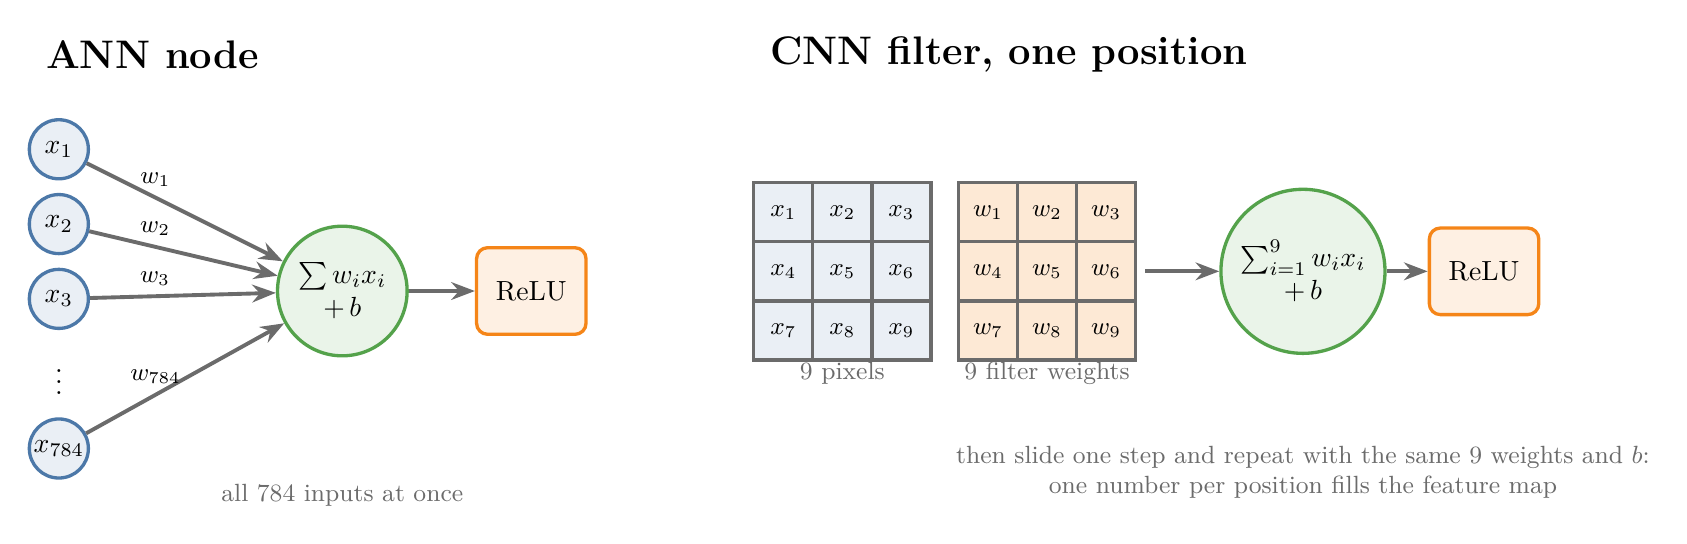
\begin{tikzpicture}[every node/.append style={font=\sffamily}]
  % ANN node
  \node[title, anchor=west] at (-0.3,3.0) {ANN node};
  \foreach \i/\lab in {0/x_1,1/x_2,2/x_3,4/x_{784}}{
    \node[circle, draw=cblue, fill=cblue!12, minimum size=0.75cm, inner sep=0pt] (in\i) at (0,1.8-\i*0.95) {$\lab$};
  }
  \node at (0,1.8-3*0.95) {$\vdots$};
  \node[circle, draw=cgreen, fill=cgreen!12, minimum size=1.6cm, align=center] (n) at (3.6,0) {$\sum w_ix_i$\\$+\,b$};
  \foreach \i/\w in {0/w_1,1/w_2,2/w_3,4/w_{784}} \draw[arrow] (in\i) -- (n) node[pos=0.35, above, font=\sffamily\small] {$\w$};
  \node[box=corange] (r) at (6.0,0) {ReLU};
  \draw[arrow] (n) -- (r);
  \node[note] at (3.6,-2.6) {all 784 inputs at once};
  % CNN filter
  \begin{scope}[xshift=9.2cm]
  \node[title, anchor=west] at (-0.3,3.0) {CNN filter, one position};
  \foreach \r in {0,1,2}{\foreach \c in {0,1,2}{
    \pgfmathtruncatemacro{\k}{3*\r+\c+1}
    \node[draw=cgrey, fill=cblue!12, minimum size=0.75cm] at (\c*0.75,1.0-\r*0.75) {\small $x_{\k}$};
  }}
  \node[note] at (0.75,-1.05) {9 pixels};
  \foreach \r in {0,1,2}{\foreach \c in {0,1,2}{
    \pgfmathtruncatemacro{\k}{3*\r+\c+1}
    \node[draw=cgrey, fill=corange!18, minimum size=0.75cm] at (2.6+\c*0.75,1.0-\r*0.75) {\small $w_{\k}$};
  }}
  \node[note] at (3.35,-1.05) {9 filter weights};
  \node[circle, draw=cgreen, fill=cgreen!12, minimum size=1.6cm, align=center] (n2) at (6.6,0.25) {$\sum_{i=1}^{9} w_ix_i$\\$+\,b$};
  \draw[arrow] (4.6,0.25) -- (n2);
  \node[box=corange] (r2) at (8.9,0.25) {ReLU};
  \draw[arrow] (n2) -- (r2);
  \node[note, align=center] at (6.6,-2.3) {then slide one step and repeat with the same 9 weights and $b$:\\one number per position fills the feature map};
  \end{scope}
\end{tikzpicture}
\end{document}
